
% Default to the notebook output style

    


% Inherit from the specified cell style.




    
\documentclass{article}

    
    
    \usepackage{graphicx} % Used to insert images
    \usepackage{adjustbox} % Used to constrain images to a maximum size 
    \usepackage{color} % Allow colors to be defined
    \usepackage{enumerate} % Needed for markdown enumerations to work
    \usepackage{geometry} % Used to adjust the document margins
    \usepackage{amsmath} % Equations
    \usepackage{amssymb} % Equations
    \usepackage{eurosym} % defines \euro
    \usepackage[mathletters]{ucs} % Extended unicode (utf-8) support
    \usepackage[utf8x]{inputenc} % Allow utf-8 characters in the tex document
    \usepackage{fancyvrb} % verbatim replacement that allows latex
    \usepackage{grffile} % extends the file name processing of package graphics 
                         % to support a larger range 
    % The hyperref package gives us a pdf with properly built
    % internal navigation ('pdf bookmarks' for the table of contents,
    % internal cross-reference links, web links for URLs, etc.)
    \usepackage{hyperref}
    \usepackage{longtable} % longtable support required by pandoc >1.10
    \usepackage{booktabs}  % table support for pandoc > 1.12.2
    \usepackage{indentfirst}
    \usepackage{amsmath}
    \usepackage{floatrow}    
    
    \definecolor{orange}{cmyk}{0,0.4,0.8,0.2}
    \definecolor{darkorange}{rgb}{.71,0.21,0.01}
    \definecolor{darkgreen}{rgb}{.12,.54,.11}
    \definecolor{myteal}{rgb}{.26, .44, .56}
    \definecolor{gray}{gray}{0.45}
    \definecolor{lightgray}{gray}{.95}
    \definecolor{mediumgray}{gray}{.8}
    \definecolor{inputbackground}{rgb}{.95, .95, .85}
    \definecolor{outputbackground}{rgb}{.95, .95, .95}
    \definecolor{traceback}{rgb}{1, .95, .95}
    % ansi colors
    \definecolor{red}{rgb}{.6,0,0}
    \definecolor{green}{rgb}{0,.65,0}
    \definecolor{brown}{rgb}{0.6,0.6,0}
    \definecolor{blue}{rgb}{0,.145,.698}
    \definecolor{purple}{rgb}{.698,.145,.698}
    \definecolor{cyan}{rgb}{0,.698,.698}
    \definecolor{lightgray}{gray}{0.5}
    
    % bright ansi colors
    \definecolor{darkgray}{gray}{0.25}
    \definecolor{lightred}{rgb}{1.0,0.39,0.28}
    \definecolor{lightgreen}{rgb}{0.48,0.99,0.0}
    \definecolor{lightblue}{rgb}{0.53,0.81,0.92}
    \definecolor{lightpurple}{rgb}{0.87,0.63,0.87}
    \definecolor{lightcyan}{rgb}{0.5,1.0,0.83}
    
    % commands and environments needed by pandoc snippets
    % extracted from the output of `pandoc -s`
    \providecommand{\tightlist}{%
      \setlength{\itemsep}{0pt}\setlength{\parskip}{0pt}}
    \DefineVerbatimEnvironment{Highlighting}{Verbatim}{commandchars=\\\{\}}
    % Add ',fontsize=\small' for more characters per line
    \newenvironment{Shaded}{}{}
    \newcommand{\KeywordTok}[1]{\textcolor[rgb]{0.00,0.44,0.13}{\textbf{{#1}}}}
    \newcommand{\DataTypeTok}[1]{\textcolor[rgb]{0.56,0.13,0.00}{{#1}}}
    \newcommand{\DecValTok}[1]{\textcolor[rgb]{0.25,0.63,0.44}{{#1}}}
    \newcommand{\BaseNTok}[1]{\textcolor[rgb]{0.25,0.63,0.44}{{#1}}}
    \newcommand{\FloatTok}[1]{\textcolor[rgb]{0.25,0.63,0.44}{{#1}}}
    \newcommand{\CharTok}[1]{\textcolor[rgb]{0.25,0.44,0.63}{{#1}}}
    \newcommand{\StringTok}[1]{\textcolor[rgb]{0.25,0.44,0.63}{{#1}}}
    \newcommand{\CommentTok}[1]{\textcolor[rgb]{0.38,0.63,0.69}{\textit{{#1}}}}
    \newcommand{\OtherTok}[1]{\textcolor[rgb]{0.00,0.44,0.13}{{#1}}}
    \newcommand{\AlertTok}[1]{\textcolor[rgb]{1.00,0.00,0.00}{\textbf{{#1}}}}
    \newcommand{\FunctionTok}[1]{\textcolor[rgb]{0.02,0.16,0.49}{{#1}}}
    \newcommand{\RegionMarkerTok}[1]{{#1}}
    \newcommand{\ErrorTok}[1]{\textcolor[rgb]{1.00,0.00,0.00}{\textbf{{#1}}}}
    \newcommand{\NormalTok}[1]{{#1}}
    
    % Define a nice break command that doesn't care if a line doesn't already
    % exist.
    \def\br{\hspace*{\fill} \\* }
    % Math Jax compatability definitions
    \def\gt{>}
    \def\lt{<}
    % Document parameters
    \title{Homework 8}
    \author{Roly Vicar\'ia \\ STAT501 Fall 2015}    
    

    % Pygments definitions
    
\makeatletter
\def\PY@reset{\let\PY@it=\relax \let\PY@bf=\relax%
    \let\PY@ul=\relax \let\PY@tc=\relax%
    \let\PY@bc=\relax \let\PY@ff=\relax}
\def\PY@tok#1{\csname PY@tok@#1\endcsname}
\def\PY@toks#1+{\ifx\relax#1\empty\else%
    \PY@tok{#1}\expandafter\PY@toks\fi}
\def\PY@do#1{\PY@bc{\PY@tc{\PY@ul{%
    \PY@it{\PY@bf{\PY@ff{#1}}}}}}}
\def\PY#1#2{\PY@reset\PY@toks#1+\relax+\PY@do{#2}}

\expandafter\def\csname PY@tok@gd\endcsname{\def\PY@tc##1{\textcolor[rgb]{0.63,0.00,0.00}{##1}}}
\expandafter\def\csname PY@tok@gu\endcsname{\let\PY@bf=\textbf\def\PY@tc##1{\textcolor[rgb]{0.50,0.00,0.50}{##1}}}
\expandafter\def\csname PY@tok@gt\endcsname{\def\PY@tc##1{\textcolor[rgb]{0.00,0.27,0.87}{##1}}}
\expandafter\def\csname PY@tok@gs\endcsname{\let\PY@bf=\textbf}
\expandafter\def\csname PY@tok@gr\endcsname{\def\PY@tc##1{\textcolor[rgb]{1.00,0.00,0.00}{##1}}}
\expandafter\def\csname PY@tok@cm\endcsname{\let\PY@it=\textit\def\PY@tc##1{\textcolor[rgb]{0.25,0.50,0.50}{##1}}}
\expandafter\def\csname PY@tok@vg\endcsname{\def\PY@tc##1{\textcolor[rgb]{0.10,0.09,0.49}{##1}}}
\expandafter\def\csname PY@tok@m\endcsname{\def\PY@tc##1{\textcolor[rgb]{0.40,0.40,0.40}{##1}}}
\expandafter\def\csname PY@tok@mh\endcsname{\def\PY@tc##1{\textcolor[rgb]{0.40,0.40,0.40}{##1}}}
\expandafter\def\csname PY@tok@go\endcsname{\def\PY@tc##1{\textcolor[rgb]{0.53,0.53,0.53}{##1}}}
\expandafter\def\csname PY@tok@ge\endcsname{\let\PY@it=\textit}
\expandafter\def\csname PY@tok@vc\endcsname{\def\PY@tc##1{\textcolor[rgb]{0.10,0.09,0.49}{##1}}}
\expandafter\def\csname PY@tok@il\endcsname{\def\PY@tc##1{\textcolor[rgb]{0.40,0.40,0.40}{##1}}}
\expandafter\def\csname PY@tok@cs\endcsname{\let\PY@it=\textit\def\PY@tc##1{\textcolor[rgb]{0.25,0.50,0.50}{##1}}}
\expandafter\def\csname PY@tok@cp\endcsname{\def\PY@tc##1{\textcolor[rgb]{0.74,0.48,0.00}{##1}}}
\expandafter\def\csname PY@tok@gi\endcsname{\def\PY@tc##1{\textcolor[rgb]{0.00,0.63,0.00}{##1}}}
\expandafter\def\csname PY@tok@gh\endcsname{\let\PY@bf=\textbf\def\PY@tc##1{\textcolor[rgb]{0.00,0.00,0.50}{##1}}}
\expandafter\def\csname PY@tok@ni\endcsname{\let\PY@bf=\textbf\def\PY@tc##1{\textcolor[rgb]{0.60,0.60,0.60}{##1}}}
\expandafter\def\csname PY@tok@nl\endcsname{\def\PY@tc##1{\textcolor[rgb]{0.63,0.63,0.00}{##1}}}
\expandafter\def\csname PY@tok@nn\endcsname{\let\PY@bf=\textbf\def\PY@tc##1{\textcolor[rgb]{0.00,0.00,1.00}{##1}}}
\expandafter\def\csname PY@tok@no\endcsname{\def\PY@tc##1{\textcolor[rgb]{0.53,0.00,0.00}{##1}}}
\expandafter\def\csname PY@tok@na\endcsname{\def\PY@tc##1{\textcolor[rgb]{0.49,0.56,0.16}{##1}}}
\expandafter\def\csname PY@tok@nb\endcsname{\def\PY@tc##1{\textcolor[rgb]{0.00,0.50,0.00}{##1}}}
\expandafter\def\csname PY@tok@nc\endcsname{\let\PY@bf=\textbf\def\PY@tc##1{\textcolor[rgb]{0.00,0.00,1.00}{##1}}}
\expandafter\def\csname PY@tok@nd\endcsname{\def\PY@tc##1{\textcolor[rgb]{0.67,0.13,1.00}{##1}}}
\expandafter\def\csname PY@tok@ne\endcsname{\let\PY@bf=\textbf\def\PY@tc##1{\textcolor[rgb]{0.82,0.25,0.23}{##1}}}
\expandafter\def\csname PY@tok@nf\endcsname{\def\PY@tc##1{\textcolor[rgb]{0.00,0.00,1.00}{##1}}}
\expandafter\def\csname PY@tok@si\endcsname{\let\PY@bf=\textbf\def\PY@tc##1{\textcolor[rgb]{0.73,0.40,0.53}{##1}}}
\expandafter\def\csname PY@tok@s2\endcsname{\def\PY@tc##1{\textcolor[rgb]{0.73,0.13,0.13}{##1}}}
\expandafter\def\csname PY@tok@vi\endcsname{\def\PY@tc##1{\textcolor[rgb]{0.10,0.09,0.49}{##1}}}
\expandafter\def\csname PY@tok@nt\endcsname{\let\PY@bf=\textbf\def\PY@tc##1{\textcolor[rgb]{0.00,0.50,0.00}{##1}}}
\expandafter\def\csname PY@tok@nv\endcsname{\def\PY@tc##1{\textcolor[rgb]{0.10,0.09,0.49}{##1}}}
\expandafter\def\csname PY@tok@s1\endcsname{\def\PY@tc##1{\textcolor[rgb]{0.73,0.13,0.13}{##1}}}
\expandafter\def\csname PY@tok@kd\endcsname{\let\PY@bf=\textbf\def\PY@tc##1{\textcolor[rgb]{0.00,0.50,0.00}{##1}}}
\expandafter\def\csname PY@tok@sh\endcsname{\def\PY@tc##1{\textcolor[rgb]{0.73,0.13,0.13}{##1}}}
\expandafter\def\csname PY@tok@sc\endcsname{\def\PY@tc##1{\textcolor[rgb]{0.73,0.13,0.13}{##1}}}
\expandafter\def\csname PY@tok@sx\endcsname{\def\PY@tc##1{\textcolor[rgb]{0.00,0.50,0.00}{##1}}}
\expandafter\def\csname PY@tok@bp\endcsname{\def\PY@tc##1{\textcolor[rgb]{0.00,0.50,0.00}{##1}}}
\expandafter\def\csname PY@tok@c1\endcsname{\let\PY@it=\textit\def\PY@tc##1{\textcolor[rgb]{0.25,0.50,0.50}{##1}}}
\expandafter\def\csname PY@tok@kc\endcsname{\let\PY@bf=\textbf\def\PY@tc##1{\textcolor[rgb]{0.00,0.50,0.00}{##1}}}
\expandafter\def\csname PY@tok@c\endcsname{\let\PY@it=\textit\def\PY@tc##1{\textcolor[rgb]{0.25,0.50,0.50}{##1}}}
\expandafter\def\csname PY@tok@mf\endcsname{\def\PY@tc##1{\textcolor[rgb]{0.40,0.40,0.40}{##1}}}
\expandafter\def\csname PY@tok@err\endcsname{\def\PY@bc##1{\setlength{\fboxsep}{0pt}\fcolorbox[rgb]{1.00,0.00,0.00}{1,1,1}{\strut ##1}}}
\expandafter\def\csname PY@tok@mb\endcsname{\def\PY@tc##1{\textcolor[rgb]{0.40,0.40,0.40}{##1}}}
\expandafter\def\csname PY@tok@ss\endcsname{\def\PY@tc##1{\textcolor[rgb]{0.10,0.09,0.49}{##1}}}
\expandafter\def\csname PY@tok@sr\endcsname{\def\PY@tc##1{\textcolor[rgb]{0.73,0.40,0.53}{##1}}}
\expandafter\def\csname PY@tok@mo\endcsname{\def\PY@tc##1{\textcolor[rgb]{0.40,0.40,0.40}{##1}}}
\expandafter\def\csname PY@tok@kn\endcsname{\let\PY@bf=\textbf\def\PY@tc##1{\textcolor[rgb]{0.00,0.50,0.00}{##1}}}
\expandafter\def\csname PY@tok@mi\endcsname{\def\PY@tc##1{\textcolor[rgb]{0.40,0.40,0.40}{##1}}}
\expandafter\def\csname PY@tok@gp\endcsname{\let\PY@bf=\textbf\def\PY@tc##1{\textcolor[rgb]{0.00,0.00,0.50}{##1}}}
\expandafter\def\csname PY@tok@o\endcsname{\def\PY@tc##1{\textcolor[rgb]{0.40,0.40,0.40}{##1}}}
\expandafter\def\csname PY@tok@kr\endcsname{\let\PY@bf=\textbf\def\PY@tc##1{\textcolor[rgb]{0.00,0.50,0.00}{##1}}}
\expandafter\def\csname PY@tok@s\endcsname{\def\PY@tc##1{\textcolor[rgb]{0.73,0.13,0.13}{##1}}}
\expandafter\def\csname PY@tok@kp\endcsname{\def\PY@tc##1{\textcolor[rgb]{0.00,0.50,0.00}{##1}}}
\expandafter\def\csname PY@tok@w\endcsname{\def\PY@tc##1{\textcolor[rgb]{0.73,0.73,0.73}{##1}}}
\expandafter\def\csname PY@tok@kt\endcsname{\def\PY@tc##1{\textcolor[rgb]{0.69,0.00,0.25}{##1}}}
\expandafter\def\csname PY@tok@ow\endcsname{\let\PY@bf=\textbf\def\PY@tc##1{\textcolor[rgb]{0.67,0.13,1.00}{##1}}}
\expandafter\def\csname PY@tok@sb\endcsname{\def\PY@tc##1{\textcolor[rgb]{0.73,0.13,0.13}{##1}}}
\expandafter\def\csname PY@tok@k\endcsname{\let\PY@bf=\textbf\def\PY@tc##1{\textcolor[rgb]{0.00,0.50,0.00}{##1}}}
\expandafter\def\csname PY@tok@se\endcsname{\let\PY@bf=\textbf\def\PY@tc##1{\textcolor[rgb]{0.73,0.40,0.13}{##1}}}
\expandafter\def\csname PY@tok@sd\endcsname{\let\PY@it=\textit\def\PY@tc##1{\textcolor[rgb]{0.73,0.13,0.13}{##1}}}

\def\PYZbs{\char`\\}
\def\PYZus{\char`\_}
\def\PYZob{\char`\{}
\def\PYZcb{\char`\}}
\def\PYZca{\char`\^}
\def\PYZam{\char`\&}
\def\PYZlt{\char`\<}
\def\PYZgt{\char`\>}
\def\PYZsh{\char`\#}
\def\PYZpc{\char`\%}
\def\PYZdl{\char`\$}
\def\PYZhy{\char`\-}
\def\PYZsq{\char`\'}
\def\PYZdq{\char`\"}
\def\PYZti{\char`\~}
% for compatibility with earlier versions
\def\PYZat{@}
\def\PYZlb{[}
\def\PYZrb{]}
\makeatother


    % Exact colors from NB
    \definecolor{incolor}{rgb}{0.0, 0.0, 0.5}
    \definecolor{outcolor}{rgb}{0.545, 0.0, 0.0}



    
    % Prevent overflowing lines due to hard-to-break entities
    \sloppy 
    % Setup hyperref package
    \hypersetup{
      breaklinks=true,  % so long urls are correctly broken across lines
      colorlinks=true,
      urlcolor=blue,
      linkcolor=darkorange,
      citecolor=darkgreen,
      }
    % Slightly bigger margins than the latex defaults
    
    \geometry{verbose,tmargin=1in,bmargin=1in,lmargin=1in,rmargin=1in}
    
    

    \begin{document}
    
    
    \maketitle
    
    

    
    \subsubsection{Question 1}\label{question-1}

\begin{enumerate}
\def\labelenumi{\alph{enumi})}
\tightlist
\item
  The plot shows a negative association between y and time. As time
increases, the y decreases. The plot also shows a curvlinear
relationship between y and time. There is also greater variance in the y
values for smaller values of time.

  \begin{figure}[h!]
 \centering
 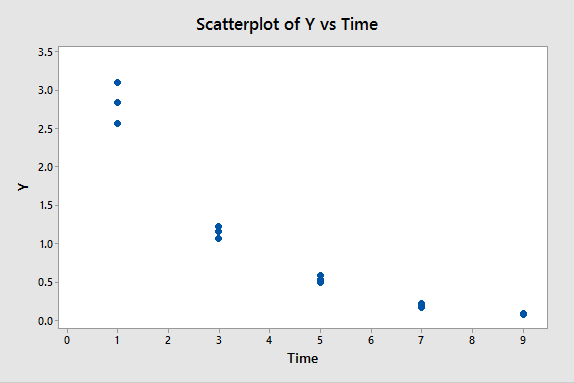
\includegraphics[scale=.5]{./images/scatterplot_y-vs-time.png}
 % scatterplot_y-vs-time.png: 574x383 pixel, 96dpi, 15.19x10.13 cm, bb=0 0 430 287
\end{figure}
\end{enumerate}

\begin{enumerate}
\def\labelenumi{\alph{enumi})}
\setcounter{enumi}{1}
\tightlist
\item
  \(Y = 2.575 - 0.3240 Time\)
  
  \begin{figure}[h!]
 \centering
 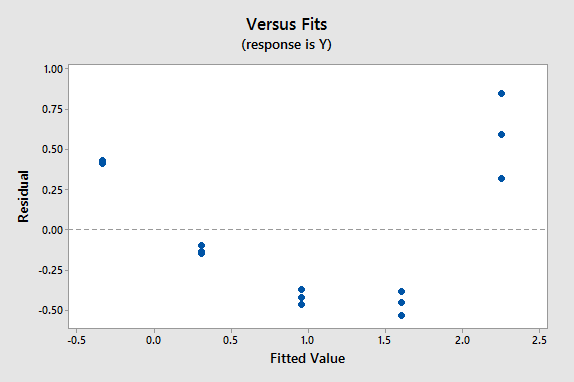
\includegraphics[scale=.5]{./images/scatterplot_residual-vs-fits_y-vs-time.png}
 % scatterplot_residual-vs-fits_y-vs-time.png: 574x382 pixel, 96dpi, 15.19x10.11 cm, bb=0 0 430 286
\end{figure}

The plot of residuals vs fitted values indicates a non-linear
relationship and non-constant variance of the errors.
\end{enumerate}

\begin{enumerate}
\def\labelenumi{\alph{enumi})}
\setcounter{enumi}{2}
\item
  Based on the two previous plots, it may be best to transform the
  y-variable in this case, because in this case there are issues with
  the linearity AND the error terms. A transformation on x primarily
  corrects the non-linearity, but does not do much to correct the
  variation of the error terms. A transformation on y corrects problems
  with the error terms and may help the non-linearity.
  
  \newpage
\item
  \(SqrtY = 1.6998 - 0.1724 Time\)
  
  \begin{figure}[!h]
  \begin{floatrow}
   \ffigbox{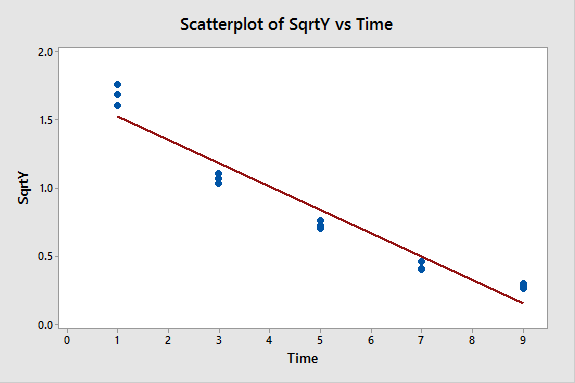
\includegraphics[scale=0.5]{./images/scatterplot_sqrty-vs-time_with_regression.png}}{}
   \ffigbox{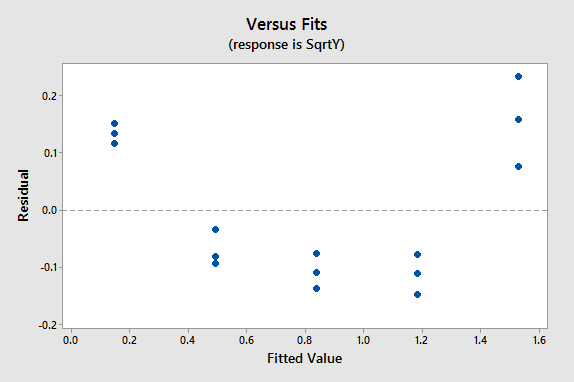
\includegraphics[scale=0.5]{./images/scatterplot_residual-vs-fits_sqrty-vs-time.png}}{}
  \end{floatrow}
\end{figure}

The plot of sqrtY vs time looks much better than the previous plot and
shows an R-sq value of 93.85\%. However, the plot of residuals versus
fitted value still shows an up-down-up pattern indicating non-linearity.
  
\end{enumerate}

\begin{enumerate}
\def\labelenumi{\alph{enumi})}
\setcounter{enumi}{4}
\tightlist
\item
  \(LnY = 1.5080 - 0.4500 Time\)
  
\begin{figure}[!h]
  \begin{floatrow}
   \ffigbox{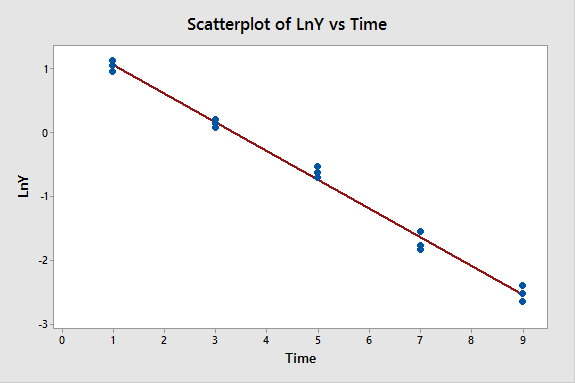
\includegraphics[scale=0.5]{./images/scatterplot_lny-vs-time_with_regression.png}}{}
   \ffigbox{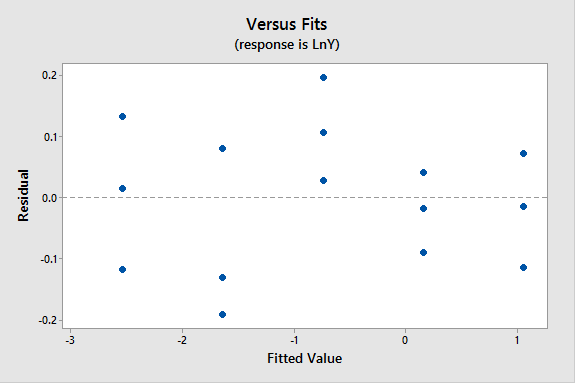
\includegraphics[scale=0.5]{./images/scatterplot_residual-vs-fits_lny-vs-time.png}}{}
  \end{floatrow}
\end{figure}
  
The plot of lnY vs time looks almost perfectly linear compared to the
previous plots and shows an R-sq value of 99.30\%. The plot of residuals
versus fitted values now shows more of a horizontal band shape with
points distributed pretty evenly above and below the residual = 0 line.
This indicates good linear fit. The error variance appears constant and
normally distributed.
\end{enumerate}

\begin{enumerate}
\def\labelenumi{\alph{enumi})}
\setcounter{enumi}{5}
\tightlist
\item
  Of the models examined, the model fitting lnY versus time is the best.
  It's residual versus fit plot showed the most constant error variance
  and normal distribution. The Ryan-Joiner test shows a high p-value so
  we fail to reject the null hypothesis that the terms are normally
  distributed. The other models all showed signs of non-linearity and
  non-constant variance of the error terms.
  
  \begin{figure}[h!]
 \centering
 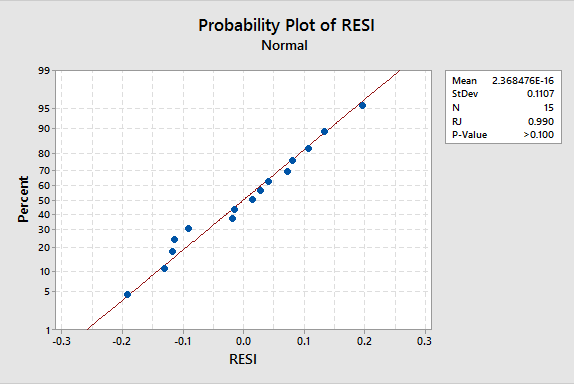
\includegraphics[scale=.4]{./images/probPlot_residual_lnY-vs-time.png}
 % probPlot_residual_lnY-vs-time.png: 574x384 pixel, 96dpi, 15.19x10.16 cm, bb=0 0 430 288
\end{figure}
\end{enumerate}

\newpage

    \subsubsection{Question 2}\label{question-2}

\begin{enumerate}
\def\labelenumi{\alph{enumi})}
\item
  \(Calories = 33.6 + 6.28 carb + 10.81 fat - 0.2053 carb*fat\)
\item
  Minitab shows a p-value of 0.034 for the estimate of \(\beta_3\). At
  the 5\% significance level, we reject the null hypothesis that
  \(\beta_3 = 0\) and conclude that \(\beta_3\) is significant. In the
  context of this problem, \(\beta_3\) signifies the effect that carb
  and fat have on Calories in the presence of each other.
\item
  \begin{enumerate}
  \def\labelenumii{\roman{enumii}.}
  \tightlist
  \item
    \(Calories = 159.2 + 6.704 fat\)
  \item
    \(Calories = 222 + 4.651 fat\)
  \item
    \(Calories = 284.8 + 2.598 fat\)
  \item
    \(Calories = 347.6 + 0.545 fat\)
  \end{enumerate}
\item
Plots of above equations for carbs = 20, 30, 40, and 50:
\begin{figure}[h!]
 \centering
 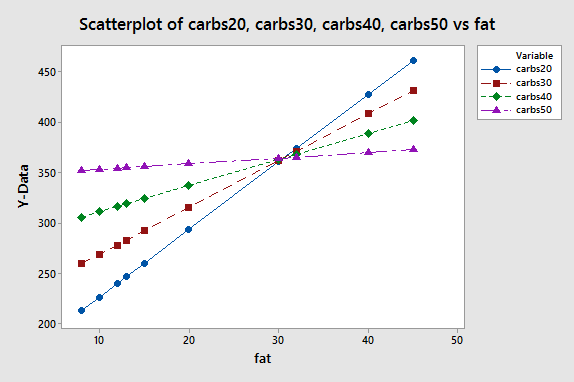
\includegraphics[scale=.5]{./images/scatterplot_carbs-vs-fat_multiple-lines.png}
 % scatterplot_carbs-vs-fat_multiple-lines.png: 574x382 pixel, 96dpi, 15.19x10.11 cm, bb=0 0 430 286
\end{figure}

\item
  The model equation estimated in part (a) shows us that the interaction
  effect between carbs and fat intake on the amount of calories
  generated is that as one of the values increases, the relative
  contribution of the other value decreases. In other words, the
  equations from part (c) showed that as we increased the value of carbs
  by units of 10, the slope on fat decreased by roughly 2.05. The lines
  showed that at higher carb values, calories hardly changed in response
  ot fat. This relationship would be similar if we fixed fat and plotted
  out functions of carbs.
\end{enumerate}

\newpage
    \subsubsection{Question 3}\label{question-3}

\begin{enumerate}
\def\labelenumi{\alph{enumi})}
\tightlist
\item
  Response variable \(y\), predictor variable \(ln(x)\): \((y_4, x_4)\)
  
  \begin{figure}[!h]
  \begin{floatrow}
   \ffigbox{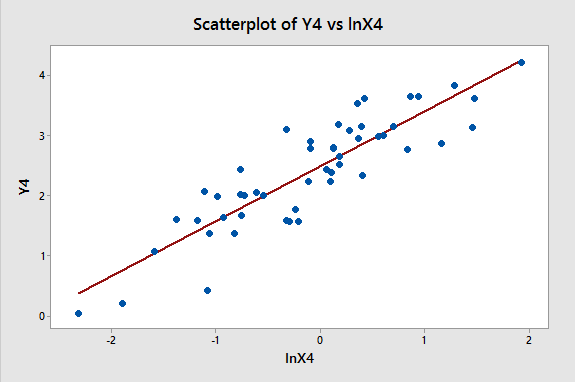
\includegraphics[scale=0.45]{./images/scatterplot_with_regression_Y4-vs-lnX4.png}}{}
   \ffigbox{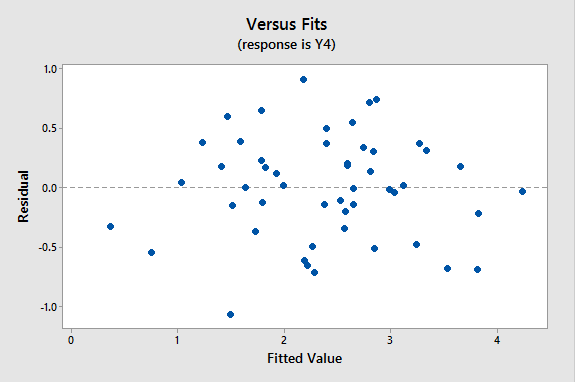
\includegraphics[scale=0.45]{./images/scatterplot_residuals-vs-fitted_Y4-vs-lnX4.png}}{}
   
  \end{floatrow}
  \begin{floatrow}
   \ffigbox{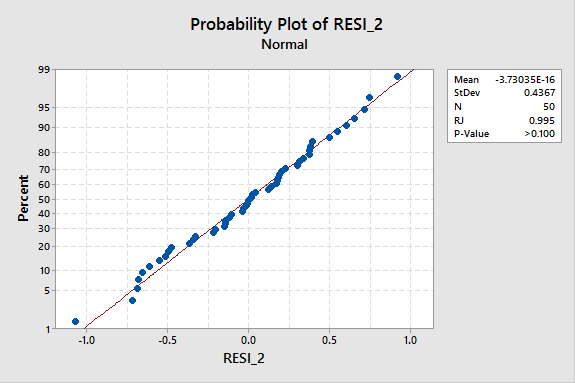
\includegraphics[scale=0.45]{./images/probPlot_residuals_Y4-vs-lnX4.png}}{}
  \end{floatrow}

\end{figure}
\end{enumerate}

\begin{enumerate}
\def\labelenumi{\alph{enumi})}
\setcounter{enumi}{1}
\tightlist
\item
  Response variable \(ln(y)\), predictor variable \(x\): \((y_3, x_3)\)
  
  \begin{figure}[!h]
  \begin{floatrow}
   \ffigbox{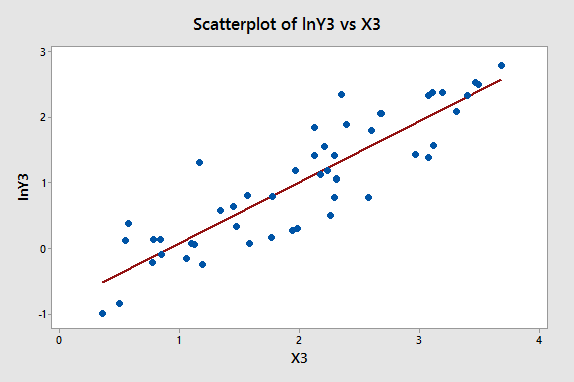
\includegraphics[scale=0.45]{./images/scatterplot_with_regression_lnY3-vs-X3.png}}{}
   \ffigbox{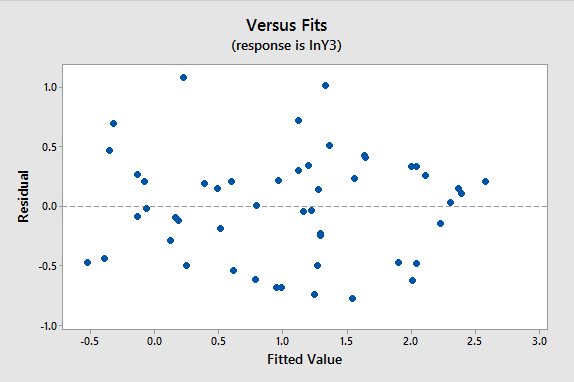
\includegraphics[scale=0.45]{./images/scatterplot_residuals-vs-fitted_lnY3-vs-X3.png}}{}
   
  \end{floatrow}
  \begin{floatrow}
   \ffigbox{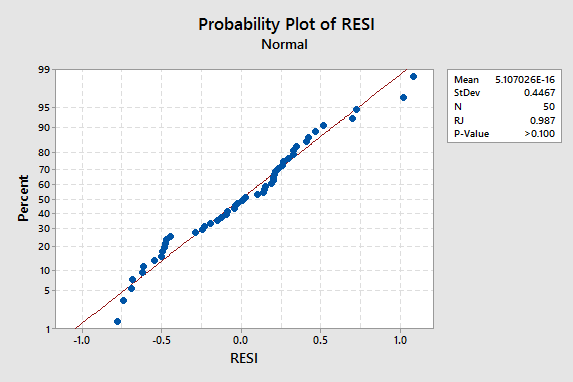
\includegraphics[scale=0.45]{./images/probPlot_residuals_lnY3-vs-X3.png}}{}
  \end{floatrow}

\end{figure}
\end{enumerate}

\newpage
\begin{enumerate}
\def\labelenumi{\alph{enumi})}
\setcounter{enumi}{2}
\tightlist
\item
  Response variable \(ln(y)\), predictor variable \(ln(x)\): \((y_1, x_1)\)
  
\begin{figure}[!h]
  \begin{floatrow}
   \ffigbox{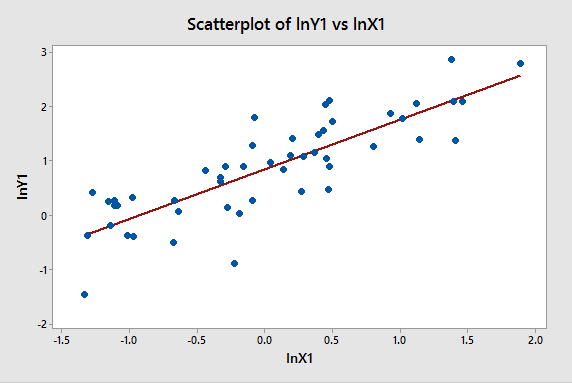
\includegraphics[scale=0.45]{./images/scatterplot_with_regression_lnY1-vs-lnX1.png}}{}
   \ffigbox{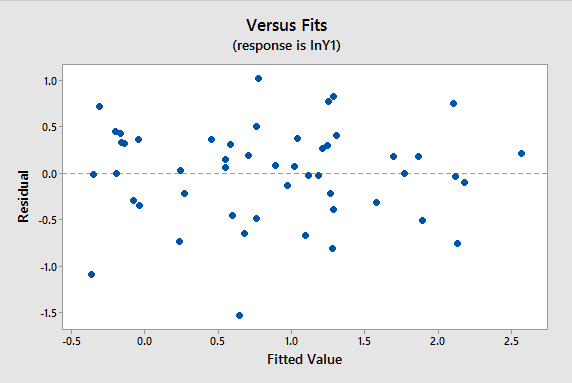
\includegraphics[scale=0.45]{./images/scatterplot_residuals-vs-fitted_lnY1-vs-lnX1.png}}{}
   
  \end{floatrow}
  \begin{floatrow}
   \ffigbox{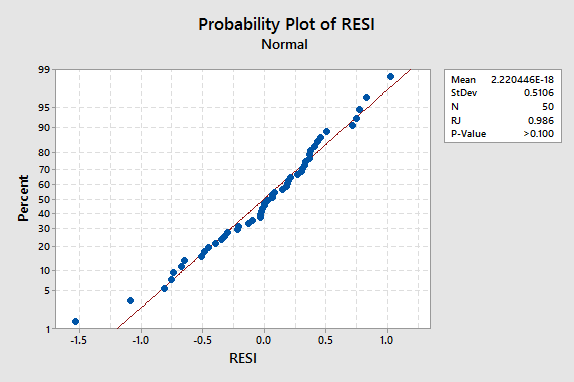
\includegraphics[scale=0.45]{./images/probPlot_residuals_lnY1-vs-lnX1.png}}{}
  \end{floatrow}

\end{figure}

\end{enumerate}

\begin{enumerate}
\def\labelenumi{\alph{enumi})}
\setcounter{enumi}{3}
\tightlist
\item
  Response variable \(y\), predictor variables \(x\) and \(x_2\): \((y_2, x_2)\)
  
\begin{figure}[!h]
  \begin{floatrow}
   \ffigbox{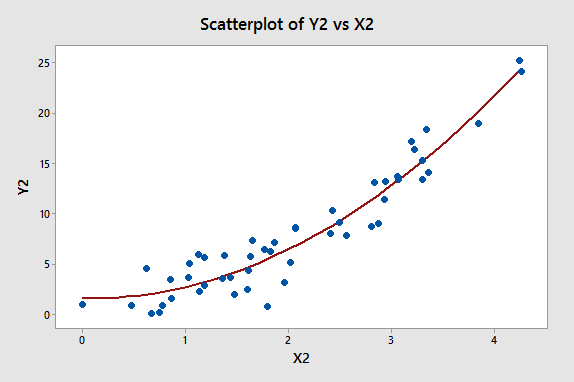
\includegraphics[scale=0.45]{./images/scatterplot_with_regression_Y2-vs-X2-and-X2-squared.png}}{}
   \ffigbox{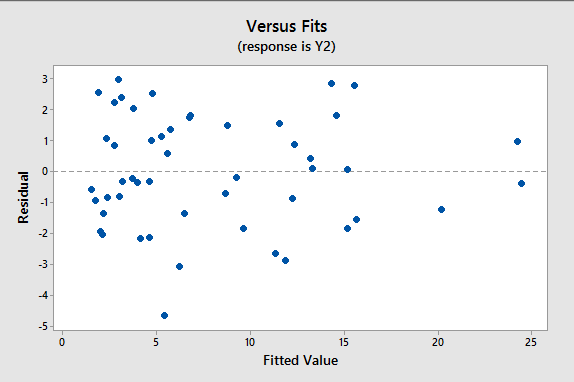
\includegraphics[scale=0.45]{./images/scatterplot_residuals-vs-fitted_Y2-vs-X2-and-X2-squared.png}}{}
   
  \end{floatrow}
  \begin{floatrow}
   \ffigbox{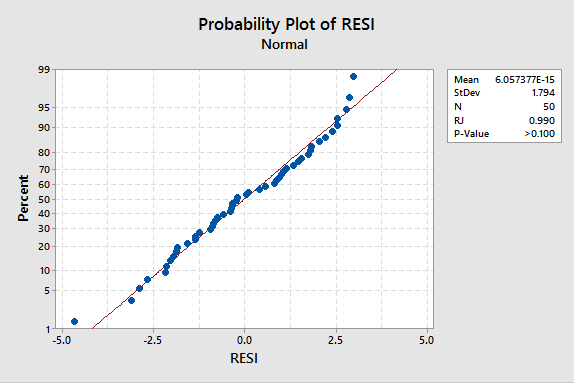
\includegraphics[scale=0.45]{./images/probPlot_residuals_Y2-vs-X2-and-X2-squared.png}}{}
  \end{floatrow}

\end{figure}
\end{enumerate}

\newpage
    \subsubsection{Question 4}\label{question-4}

\begin{enumerate}
\def\labelenumi{\alph{enumi})}
\item
  \(Velocity = 1.288 + 25.65 Concentration - 56.5 Concentration^2\)
\item
  Test statistic: t-statistic = -3.33, d.f. = 5, p-value = 0.029. The
  p-value indicates that at significance level of less than .05, we can
  reject the null hypothesis that \(\beta_2 = 0\) and conclude that
  \(\beta_2 \ne 0\). In the context of this problem, it indicates that
  velocity has a significant relationship to the square of
  concentration.
\item
The plot of residuals vs fitted values for the quadratic model shows a
down-up-down pattern which points to an obvious violation of the
linearity assumption.

\begin{figure}[h!]
 \centering
 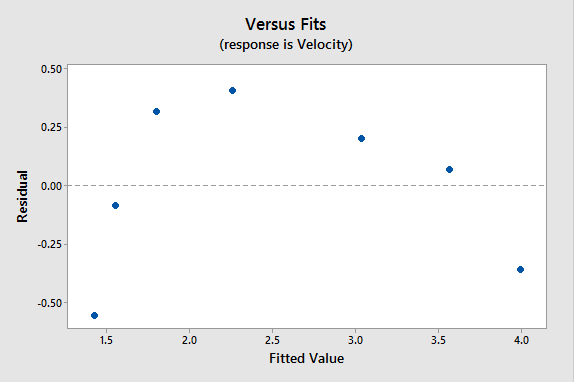
\includegraphics[scale=.5]{./images/scatterplot_residuals-vs-fitted_velocity-vs-concentration-quadratic.png}
 % scatterplot_residuals-vs-fitted_velocity-vs-concentration-quadratic.png: 574x382 pixel, 96dpi, 15.19x10.11 cm, bb=0 0 430 286
\end{figure}

\end{enumerate}

\begin{enumerate}
\def\labelenumi{\alph{enumi})}
\setcounter{enumi}{3}
\tightlist
\item
  \(Velocity = 3.920 + 0.048 lnConc - 0.1041 lnConc*lnConc\)
  
  \begin{figure}[h!]
 \centering
 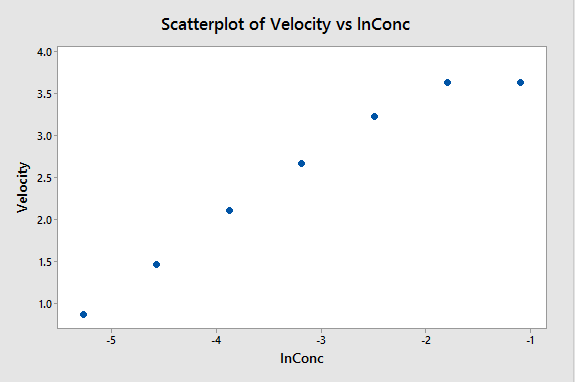
\includegraphics[scale=.5]{./images/scatterplot_velocity-vs-lnConc.png}
 % scatterplot_velocity-vs-lnConc.png: 575x382 pixel, 96dpi, 15.21x10.11 cm, bb=0 0 431 286
\end{figure}
\end{enumerate}

\begin{enumerate}
\def\labelenumi{\alph{enumi})}
\setcounter{enumi}{4}
\item
  Test statistic: t-statistic = -4.04, d.f. = 5, p-value = 0.016. The
  p-value indicates that at significance level of less than .05, we can
  reject the null hypothesis that \(\beta_2 = 0\) and conclude that
  \(\beta_2 \ne 0\). In the context of this problem, it indicates that
  velocity has a significant relationship to the square of the natural
  log of concentration.
\item
  The 95\% prediction interval for velocity at a concentration level of
  \(e^{-3}\) is (2.47741, 3.20441). This can be interpreted as saying
  that we can be 95\% confident that the velocity of a chemical reaction
  involving a concentration level \(e^{-3}\) of substrate will be
  between 2.47741 and 3.20441.
\end{enumerate}


    % Add a bibliography block to the postdoc
    
    
    
    \end{document}
